\documentclass[letterpaper]{report}
\usepackage{longtable}
\usepackage{graphicx}
\usepackage{listingsutf8}
\usepackage{pdfpages}
\usepackage{xcolor}
\usepackage[utf8]{inputenc}
\usepackage[T1]{fontenc}

\title{ Progetto di Basi di Dati \newline \begin{center}
  \textbf{Servizio di Live Streaming}
\end{center}}
\author{Francesco Mauro\footnote{Numero di matricola: 949471} , Riccardo Oro\footnote{Numero di matricola: 9494073}}
\date{2023}

\lstset{
    language=SQL,
    backgroundcolor=\color{lightgray},
    basicstyle=\scriptsize\ttfamily,
    keywordstyle=\color{blue},
    commentstyle=\color{gray},
    numberstyle=\color{green},
    stringstyle=\color{teal},
    numbers=left,
    numberstyle=\tiny\color{gray},
    breaklines=true,
    breakatwhitespace=true,
    showstringspaces=false,
    tabsize=2,
}

\begin{document}

\maketitle
\tableofcontents

\chapter{Requisiti Iniziali}
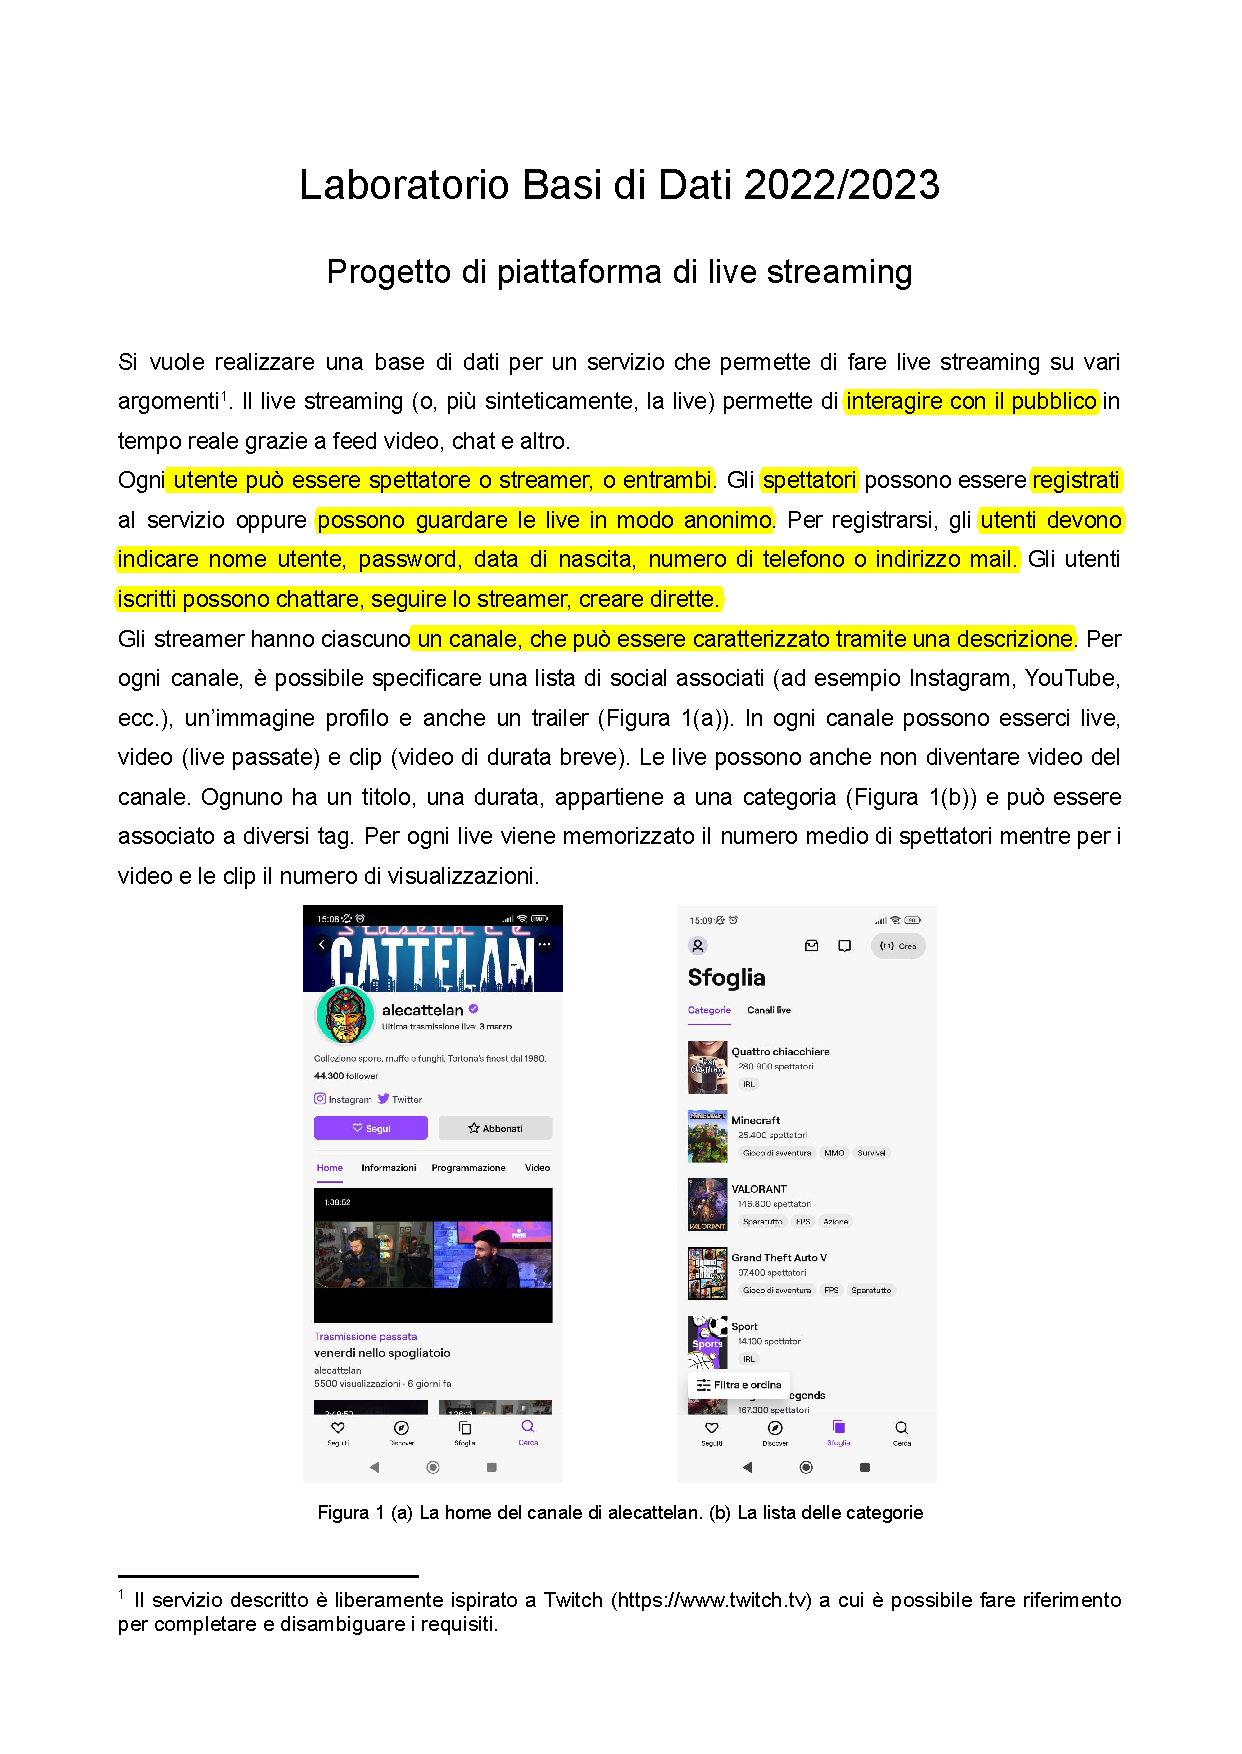
\includepdf[pages=-]{../utils/esame_progettazione_requisiti.pdf}
\chapter{Progettazione Concettuale}
\section{Glossario}

% make a table containing this fields: Termine Descrizione Sinonimi Collegamenti
\begin{center}
  
  \begin{tabular}{|p{3cm}|p{3cm}|p{3cm}|p{3cm}||}
    \hline
    Termine &Descrizione & Sinonimi &Collegamento \\
    \hline
    Utente& Chi usufruisce del servizio & Spettatore, Streamer & Spettatore, Streamer, Registrato, Anonimo \\
    \hline
    Spettatore & Colui che guarda le live & Utente & Registrato, Anonimo \\ 
    \hline
    Streamer & Colui che gestisce un canale e intrattiene gli spettatori & &Utente, Registrato, Canale\\
    \hline
    Registrato & Utente che ha fornito nome utente, password,data di nascita e numeo di telefono o indirizzo email & &Utente \\
    \hline
    Live Streaming & Trasmissione in dirtetta che permette di interagire con il pubblico in tempo reale &  & Canale, Streamer \\ 
    \hline
    Canale & Ogni streamer ha un canale dove può caricare i suoi contenuti e eventuali informazioni esterne & & Streamer, Live Streaming \\
    \hline
  \end{tabular}
  
  \end{center}
\section{Revisione dei requisiti}

\subsection{Fase relativa agli utenti}
\begin{itemize}
  \item Gli utenti si dividono in registrati o anonimi
\end{itemize}
\subsection{Fase relativa a utenti anonimi}
\begin{itemize}
  \item Gli utenti anonimi possono visitare i canali senza doversi per 
  forza regstrare, ma non possono interagire 
\end{itemize}
\subsection{Fase relativa a utenti registrati}
\begin{itemize}
  \item Gli utenti per registrarsi devono:
  \begin{itemize}
    \item Registrarsi fornendo: username,passowrd, email o numero di telefono, data di nascita
  \end{itemize}
  E possono accedere a:
    \begin{itemize}
      \item Canale 
      \item chat privata o publica
      \item portafoglio (per eventuali donazioni)
      \item possono diventare \textit{supporter} tramite \textit{subscription}
    \end{itemize} 
  Per utenit che creano contenuti invece:
    \begin{itemize}
      \item Il numero di live effettuate 
      \item il numero di minuti trasmessi
      \item il numero medio di spettatori \footnote{Tutti questi dati si possono usare per far diventare uno \textit{streamer affiliate}} %TODO: questo si può vedere anche come vincolo%
    \end{itemize}
\end{itemize}
\subsection{Fase relativa al canale}
Un canale è composto da:
\begin{itemize}
  \item Descrizione
  \item Lista dei social
  \item Immagine del profilo
  \item Trailer 
  \item Live 
  \item Video e clip \footnote{Queste non sono in streaming ma vengono salvate}
  \item Ore di streaming
\end{itemize}
\subsection{Fase relativa alle live}
\begin{itemize}
  \item Possono essere viste da tutti gli utenti
  \item Iniziano a un determinato orario
  Viene memorizzato:
    \begin{itemize}
      \item Il numero medio di spettatori
      \item Chat 
      \item il titolo
    \end{itemize}
    \item A ogni live corrisponde un URL
\end{itemize}
\subsubsection{Fase relativa a una chat}
\begin{itemize}
  \item Solo gli utenti registrati possono accedere alla chat
  Può essere:
  \begin{itemize}
    \item Privata (Tra utente e utente)
    \item Pubblica 
  \end{itemize}
\end{itemize}
\subsection{Fase relativa alle Operazioni}
\begin{itemize}
  \item Registrazione utente
  \item donazioni \footnote{A utenti registrati}
  \item Diventare follower di un canale
  \item Avviare una chat privata tra utenti registrati
\end{itemize}

\section{Schema E-R + business rules }
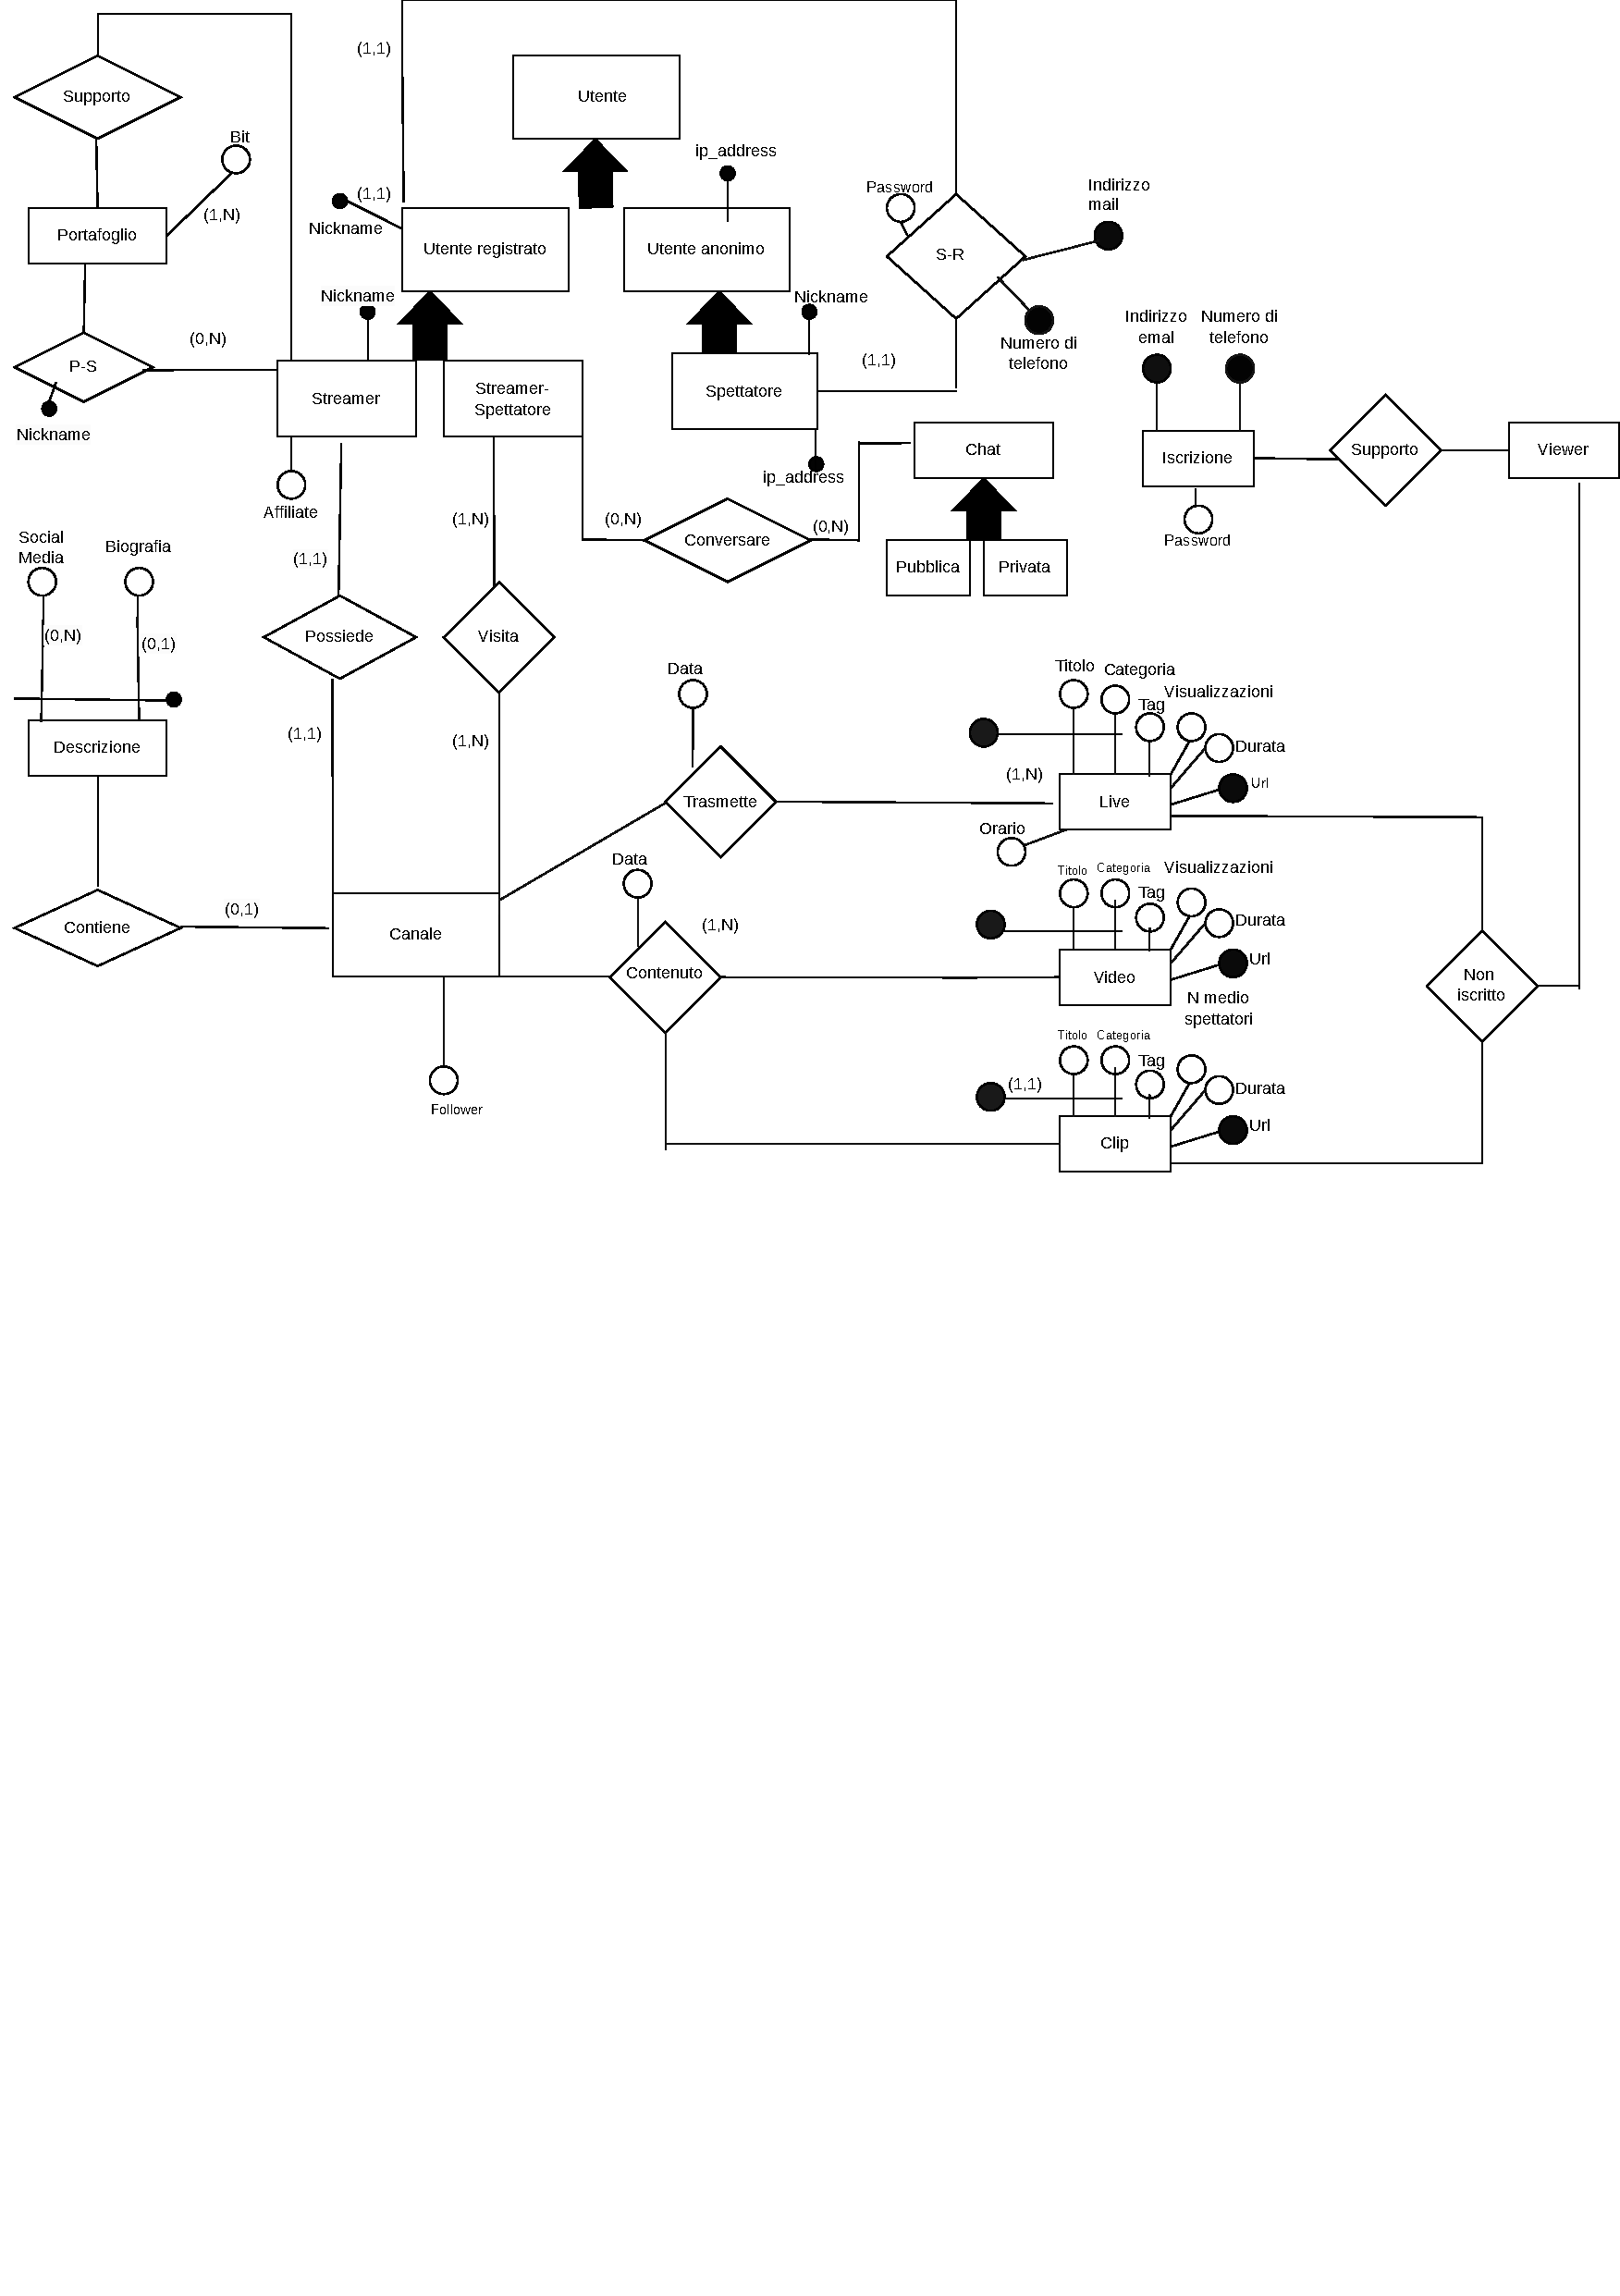
\includegraphics[width=\textwidth]{resources/schema_e-r.pdf}
\begin{itemize}
    \item I video sono degli estratti di live passate.
    \item Le clip sono dei video di breve durata.
    \item La moneta virtuale utilizzata è il bit, che può essere acquistato nella piattaforma.
    \item Un utente per registrarsi sulla piattaforma deve fornire indirizzo email o numero di telefono.
    \begin{itemize}
        \item Un utente anonimo può guardare la live trasmessa dallo streamer ma non può interagire con esso. 
    \end{itemize}
        \item Se uno \textit{streamer} rispetta i \textit{parametri di performance} può diventare \textit{affiliate}.
        \item Il portafoglio è costituito da \textit{bit}, con i quali il \textbf{follower}\footnote{solo il follower e non il viewer} può supportare lo streamer
        \item La chat permette agli utenti di comunicare l'uno con l'altro sia pubblicamente sia privatamente.
        \item Il nome del canale è lo stesso nome che l'utente inserisce durante la registrazione alla piattaforma.
\end{itemize}

\chapter{Progettazione Logica}
\section{Tavola dei volumi}
\small
\begin{longtable}{ |l|c|c|p{6.2cm}|}
  \hline \textbf{Concetto} & \textbf{Tipo} & \textbf{Volume} & \textbf{Motivazione} \\\hline
  \endfirsthead

  \hline \textbf{Concetto} & \textbf{Tipo} & \textbf{Volume} & \textbf{Motivazione} \\\hline
  \endhead

  \hline \multicolumn{4}{|r|}{\textit{Continua alla pagina successiva}}
  \endfoot

  \hline
  \endlastfoot

  Spettatore  & E & 1.000.000 & Si ipotizza un totale di 1.000.000 spettatori \\\hline
  Utenti Registrato & E & 950.000 & Si ipotizza che la maggior parte degli utenti sia registrata \\\hline
  Utenti Anonimi & E & 50.000 & Una minima parte degli spettatori non è Registrato \\\hline
  Streamer-Spetttore & E & 100.000 & Si ipotizza che 100.000 spettatori siano anche streamer \\\hline
  Streamer & E & 10.0000 & Utenti che decidono di svolgere attivita streaming sulla piattaforma\\\hline
  Descrizione & E & 10.000 & Il numero di descrizioni è pari al numero di descrizioni \\\hline
  Canali & E & 10.000 & Utenti registrati alla piattaforma e che hanno un canale attivo\\\hline
  Video & E & 100.000 & Contenuto video caricato sul canale dello streamer\\\hline
  Live & E & 1.000.000 &Contenuto video live in onda sul canale in tempo reale o live passata\\\hline
  Clip & E & 100.000 & Estratto di breve durata del contenuto in live\\\hline
  Portafoglio & E & 1000000 & Quantitivo di moneta virtuale "bit" acquistabile sulla piattaforma\\\hline
  Iscrizione & E & 750.000 & Supponiamo che 750.000 spettatori si iscrivano almeno a un canale \\\hline
  Chat & E & 1.000.000.000 &Supponiamo che vengano mandati 1.000.000.000 di messaggi tra privati e pubblici \\\hline
  Conversare & R &1.000.000.000 & Quantitivo di messaggi scambiati su chat pubbliche o private tra utenti\\\hline
  Contenuto & R & 1.200.000 & Il numero di contenuti è pari alla somma dei volumi di live video e clip  \\\hline %TODO pensare a un numero %
  Visita & R & 1.200.000& Il numero di visite è pari alla somma dei volumi di live video e clip \\\hline %TODO pensare a un numero %
  P-S & R &1.000.000 & Relazione tra Portafoglio e streamer \\\hline 
  S-R & R & 1.000.000 & Relazione utente Spettatore non registrato si registra alla piattaforma\\\hline
  Non iscritto & R & 1.000.000.000 & Utenti non registrati sulla piattaforma\\\hline
  Possiede & R & 10.000 &Quantitivo di canali complessivi presenti sulla piattaforma \\\hline
  Contiente & R & 1.200.000&Quantitivo di contenuti video presenti sulla piattaforma \\\hline
  Supporto & R & 1.300.000 &Quantitivo di supporto monetario ricevuto dallo streamer \\\hline

\end{longtable}
\normalsize

\section{Operazioni Previste}
\begin{enumerate}
    \item \textbf{Registrazione}: 
    \item \textbf{Visualizzazione Chat}:
    \item \textbf{Visualizzazione Live}: 
    \item \textbf{Visualizzazione Video}:
    \item \textbf{Visualizzazione Clip}: 
    \item \textbf{Visualizzazione Chat}: 
    \item \textbf{Visualizzazione Descrizione}:
    \item \textbf{Donazione}:
    \item \textbf{Visualizzazione Canale}
    \item \textbf{Calcolo Numero Spettatori Medi}:
    \item \textbf{Calcolo Donazioni Ricevute}: 
    \item \textbf{Calcolo Numero di live effettuate} 
    \item \textbf{Calcolo Numero di video effettuate} 
    \item \textbf{Calcolo Numero di clip effettuate} 
\end{enumerate}
%TODO: partere non in grassetto da spostare in altra tabella %
\subsection{Tavola delle operazioni}
\small
\begin{longtable}{|l|c|c|p{2.5cm}|c}
  \hline \textbf{Operazioni} & \textbf{Tipo} & \textbf{Frequenza} & \textbf{Motivazione} \\\hline
  \endfirsthead

  \hline \textbf{Operazioni} & \textbf{Tipo} & \textbf{Frequenza} & \textbf{Motivazione} \\\hline
  \endhead

  \hline \multicolumn{3}{|r|}{\textit{Continua alla pagina successiva}}
  \endfoot
  
  \hline
  \endlastfoot

  Registrazione & I & 3.000/giorno & un utente può registrarsi alla piattaforma inserendo i propri dati personali \\\hline
  Visualizzazione Clip & I & 50.000/giorno & un utente può visualizzare una clip  \\\hline
  Visualizzazione Live & I & 30.000/giorno & un utente può visualizzare una live  \\\hline
  Visualizzazione Video & I & 30.000/giorno & un utente può visualizzare un video  \\\hline
  Visualizzazoine Chat & I & 1.000.000/giorno & un utente può visualizzare la chat  \\\hline
  Donazione & I & 10.000/giorno & un utente può donare ad uno streamer  \\\hline
  Acquisto moneta \textbf{bit} da utente &I&1.000.000/settimana&un utente può acquistare \textbf{bit}. \\\hline
  Calcolo Numero Spettatori Medi & I & 1/giorno  & la piattaforma calcola il numero di spettatori medi  \\\hline
  Calcolo Numero di Live effettuate & I & 1/giorno  & la piattaforma calcola il numero di live effettuate da uno streamer  \\\hline
  Calcolo Numero di Clip effettuate & I & 1/giorno  & la piattaforma calcola il video di live effettuate da uno streamer  \\\hline
  Calcolo Numero di Video effettuate & I & 1/giorno  & la piattaforma calcola il clip di live effettuate da uno streamer  \\\hline
  Controllo condizioni affiliate & B &1/giorno & la piattaforma controlla se uno streamer rispetta le condizioni per diventare affiliate  \\\hline
  Controllo classifica streamer più seguiti & B & 1/settimana  & la piattaforma controlla se uno streamer rispetta le condizioni per diventare affiliate. \\\hline
  Calcolo numero iscrizioni al canale &B&1/giorno&La piattaforma calcola quanti utente hanno deciso di seguire il canale dello streamer.\\\hline
  Calcolo numero \textbf{bit} acquistati dagli utenti &B& 1/giorno &La piattaforma calcola il totale di \textbf{bit} acquistati dagli utenti e inseriti nel Portafogli.\\\hline
\end{longtable}
\normalsize

\section{Ristrutturazione schema E-R}
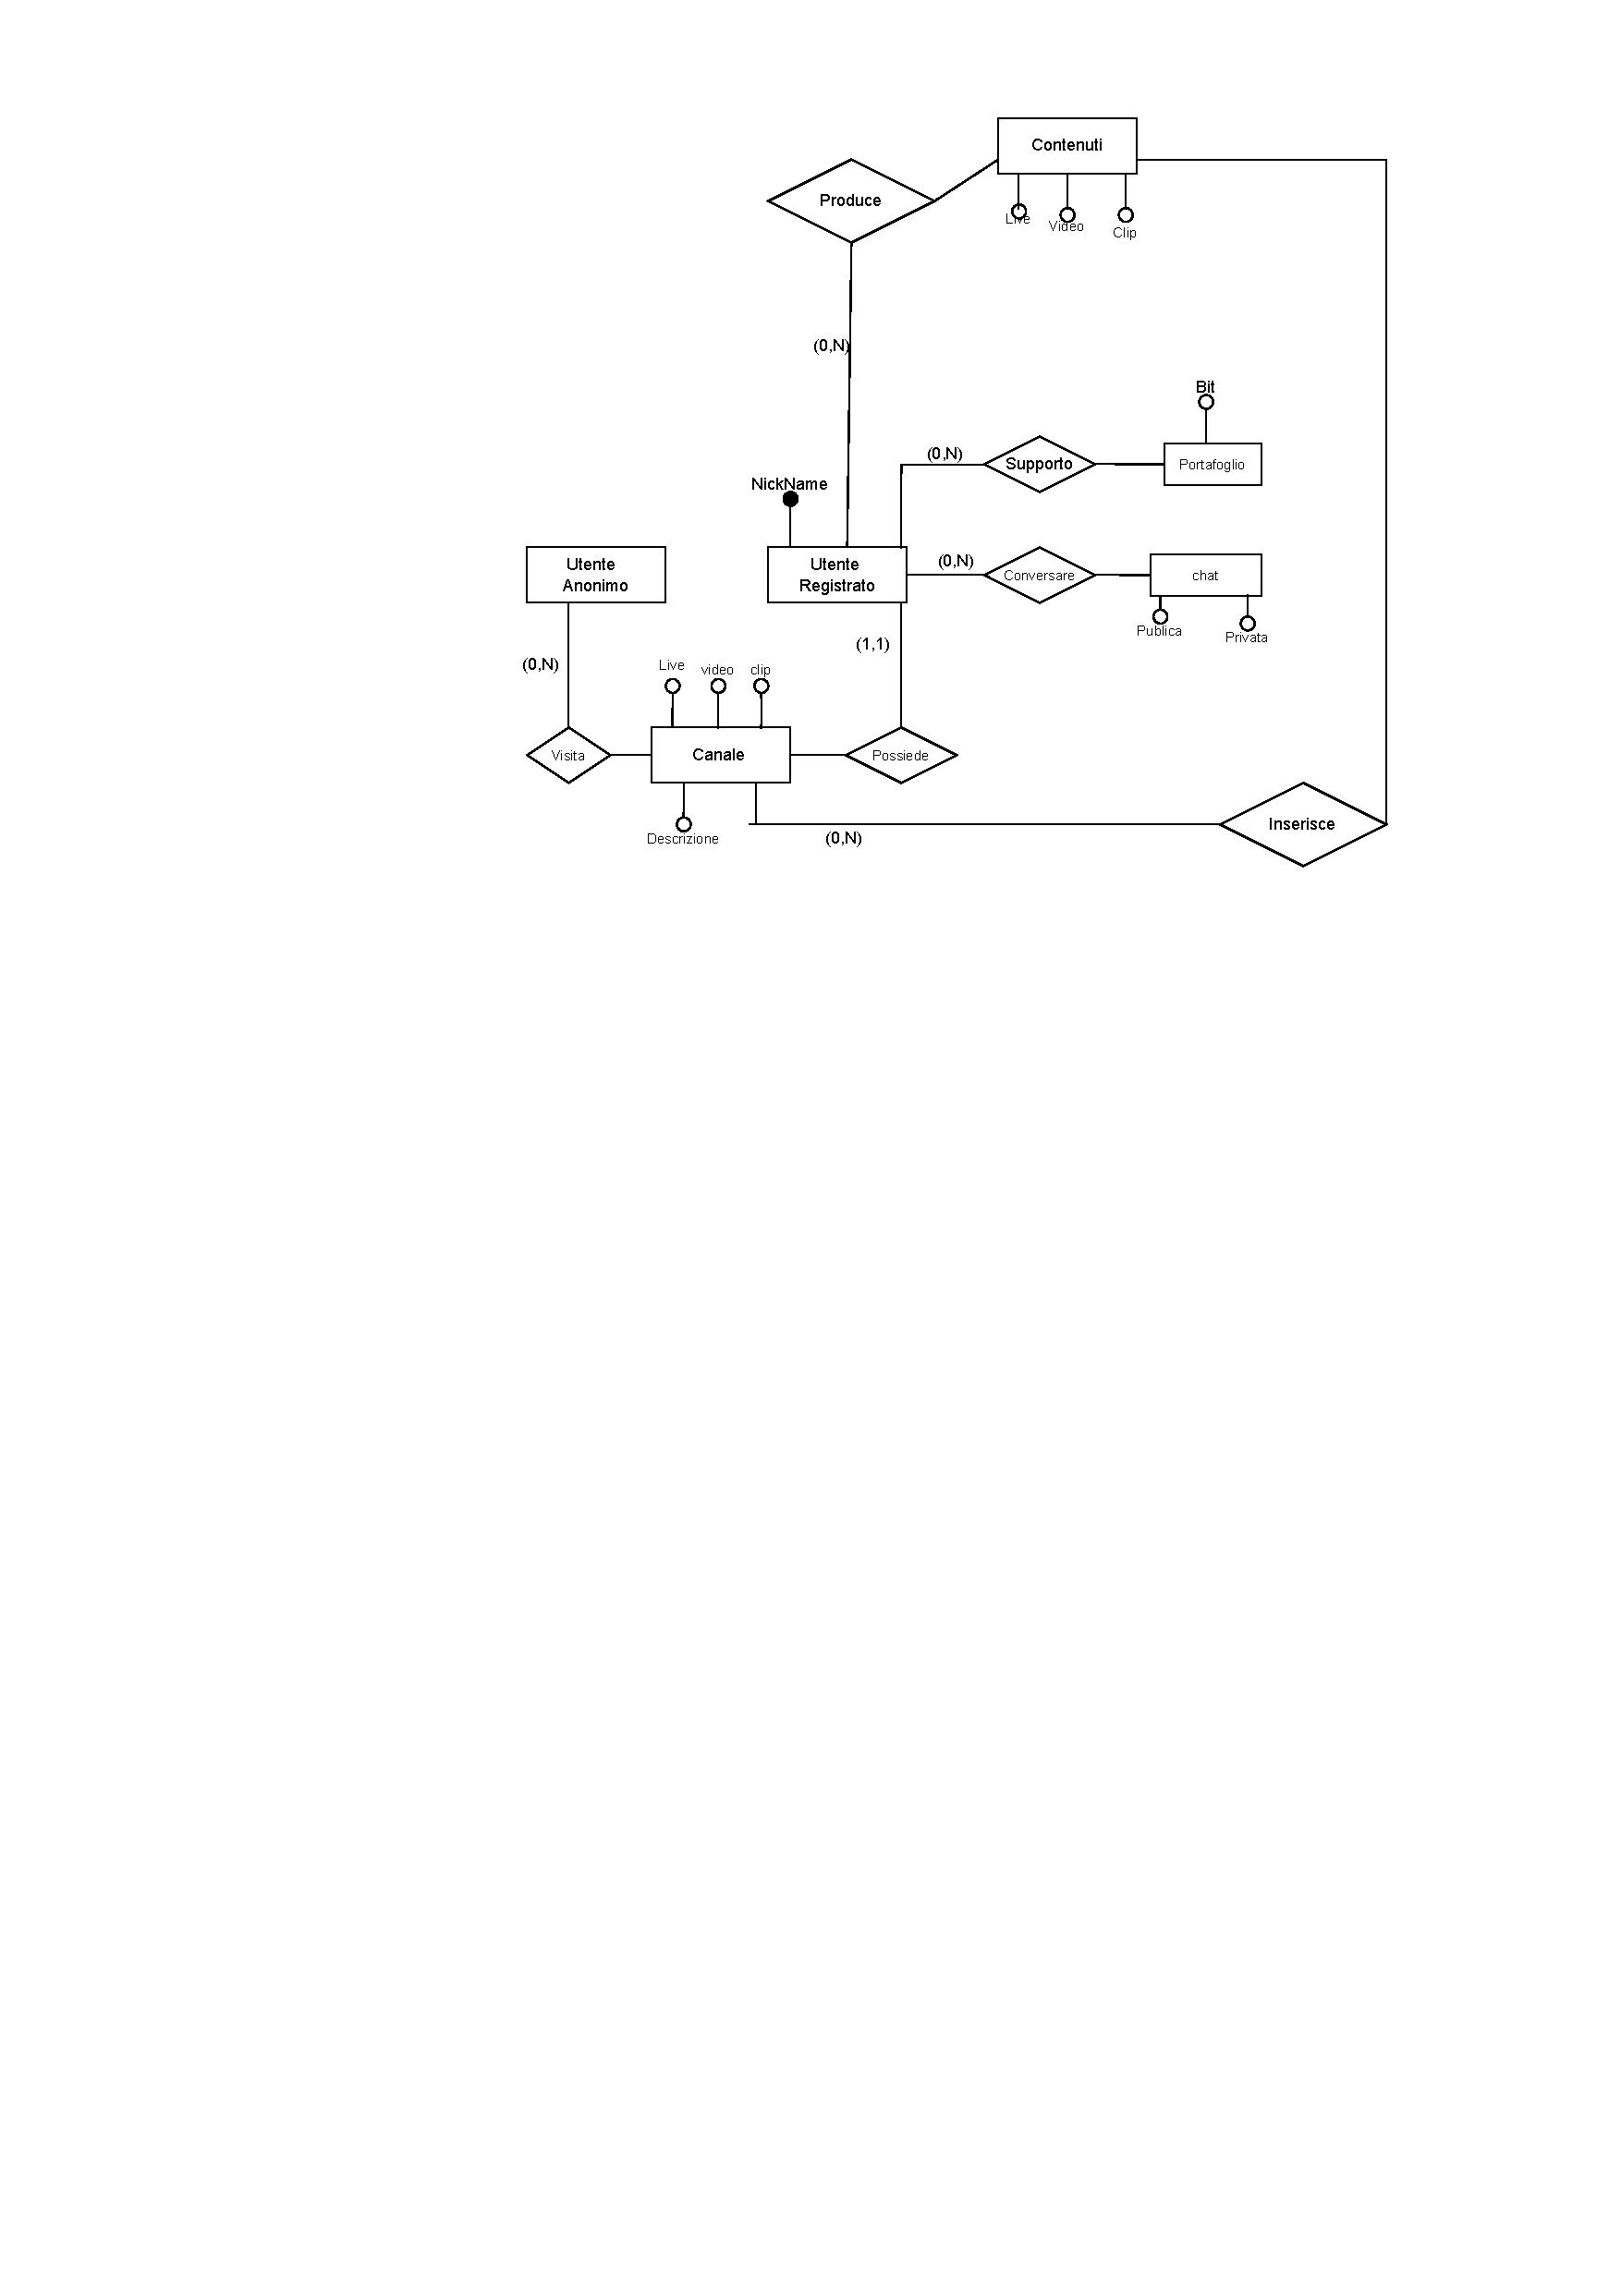
\includegraphics[width=\textwidth]{resources/e_r_ridotto.pdf}

\section{Analisi delle Generalizzazioni}
Le generalizzazioni presenti nello schema E-R sono:
\begin{enumerate}
    \item \textbf{Utente}: È una generalizzazione totale tra le entità \textit{Utente registrato} e \textit{Utente anonimo}, poichè o si è registrati alla piattaforma o si è anonimi
    \item \textbf{Streamer e Streamer-Spettatore}: È una generalizzazione parziale tra le entità \textit{Streamer} e \textit{Streamer-Spettatore}, in quanto l'utente registrato si ritrova a svolgere il ruolo o di streamer o di spettatore, ma sempre essendo uno streamer  
    \item \textbf{Spettatore - Utente Anonimo}: È una generalizzazione sovrapposta, poiché l'utente anonimo può essere solo spettatore'
    \item \textbf{Chat}: È una generalizzazione totale tra le entità \textit{Chat privata} e \textit{Chat pubblica}. Perché l'entià chat si divide in due sottoinsiemi, ovvero chat pubblica e chat privata.
\end{enumerate} 
\section{Partizionamento/Accorpamento di entità e associazioni}
Si è deciso di accorpare l'entità chat, così indica in maniera più coincisa che un utente registrato può comunicare in maniera pubblica o privata'''
\begin{figure}[ht]
    \centering
    \begin{minipage}{.45\textwidth}
        \centering
        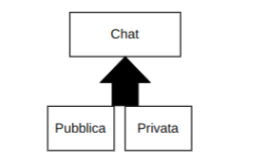
\includegraphics[width=0.9\linewidth]{resources/chat_revised.png}
        \caption{Entità chat dopo l'accorpamento}
        \label{Entità chat dopo l'accorpamento}
    \end{minipage}%
    \begin{minipage}{.5\textwidth}
        \centering
        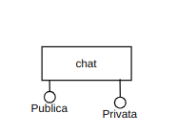
\includegraphics[width=0.9\linewidth]{resources/chat.png}
        \caption{Entità chat prima dell'accorpamento}
        \label{Entità chat prima dell'accorpamento}
    \end{minipage}
\end{figure}

\section{Business rules dell'E-R ristrutturato }
\begin{itemize}
    \item Gli attributi live ,video ,clip presenti nell'entità \textbf{canale} indicato un oggetto finito e caricato al suo interno.
    \item Gli attributi live ,vide ,clip presenti sull'entitá \textbf{contenuti} indicano un oggetto che ancora o è in fase di produzione o è un prodotto finito ma non caricato sul canale del proprietario. 
    \item Gli utenti anonimi non possono supportare gli streamer. 
    \item Gli streamer sono utenti registrati che caricano  o trasmettono contenuti. 
    \item Ogni utente registrato ha un nickname. 
    \item Il nickname scelto dall'utente registrato sarà anche il nome del canale. 
    \item Ogni canale ha una Descrizione. 
    \item Le live sono contenuti o in tempo reale.
    \item I video sono live già concluse. 
    \item Le clip sono brevi estratti di video. 
    \item Un utente anonimo non può conversare con altri utenti.
    \item Un utente anonimo non possiede un canale. 
\end{itemize}

\section{Schema Relazionale}
\begin{itemize}
    \item Utente registrato(\underline{nickname},\underline{email},password,affiliato,numero di telefono)
    \item Utente anonimo(\underline{ip address}).
    \item Canale(live, video , clip,n\_iscritti,\underline{nickname},iscritti).
    \item Descrizione(\underline{Nome},link\_social,biografia) 
    \item Calendario(\underline{timestamp\_inizio,titolo\_futuro})
    \item Contenuti(\underline{Url},live ,video , clip).
    \item Portafoglio(bit,\underline{nickname}). 
    \item Chat(\underline{UID messaggio},pubblica ,privata, nickname mandante ,nickname ricevente). 
    \item struttura(visibilità , data, categoria , \underline{titolo ,durata}, tag)
    \item Visita(\underline{utente anonimo} ,canale).
    \item Possiede(\underline{utente registrato},canale).
    \item Inserisce(canale,\underline{contenuti}).
    \item Produce(\underline{utente registrato},contenuti).
    \item Supporto(\underline{utente registrato} ,portafoglio).
    \item Conversare(\underline{utente registrato} ,chat).
    \item Impostato(\underline{struttura} ,contenuti)
\end{itemize}
\chapter{DDL di creazione del DB}
\section{DDL per il Canale}
\lstinputlisting{sql/DDL/canale.sql}
\lstinputlisting{sql/DDL/streamer.sql}
\lstinputlisting{sql/DDL/utente.sql}
\lstinputlisting{sql/DDL/spettatore.sql}
\lstinputlisting{sql/DDL/utente_anonimo.sql}
\newpage
\lstinputlisting{sql/DDL/utente_registrato.sql}
\lstinputlisting{sql/DDL/descrizione.sql}
\lstinputlisting{sql/DDL/chat.sql}
\lstinputlisting{sql/DDL/video.sql}

\end{document}